\documentclass{article}
\usepackage{listings}
\usepackage{pythonhighlight}
\usepackage{graphicx}

\lstdefinestyle{BashOutputStyle}{
  basicstyle=\footnotesize\ttfamily,
  numbers=none,
  frame=tblr,
  columns=fullflexible,
  backgroundcolor=\color{blue!10},
  linewidth=0.9\linewidth}
  
\begin{document}

\noindent In all examples, assume that the HEC-RAS data has already been imported as a DataFrame called \texttt{riverData}.

\section*{Plotting metrics with no optional inputs}

\begin{python}
plotHECRAS(riverData, 'Q')
\end{python}

\begin{figure}[h]
    \centering
    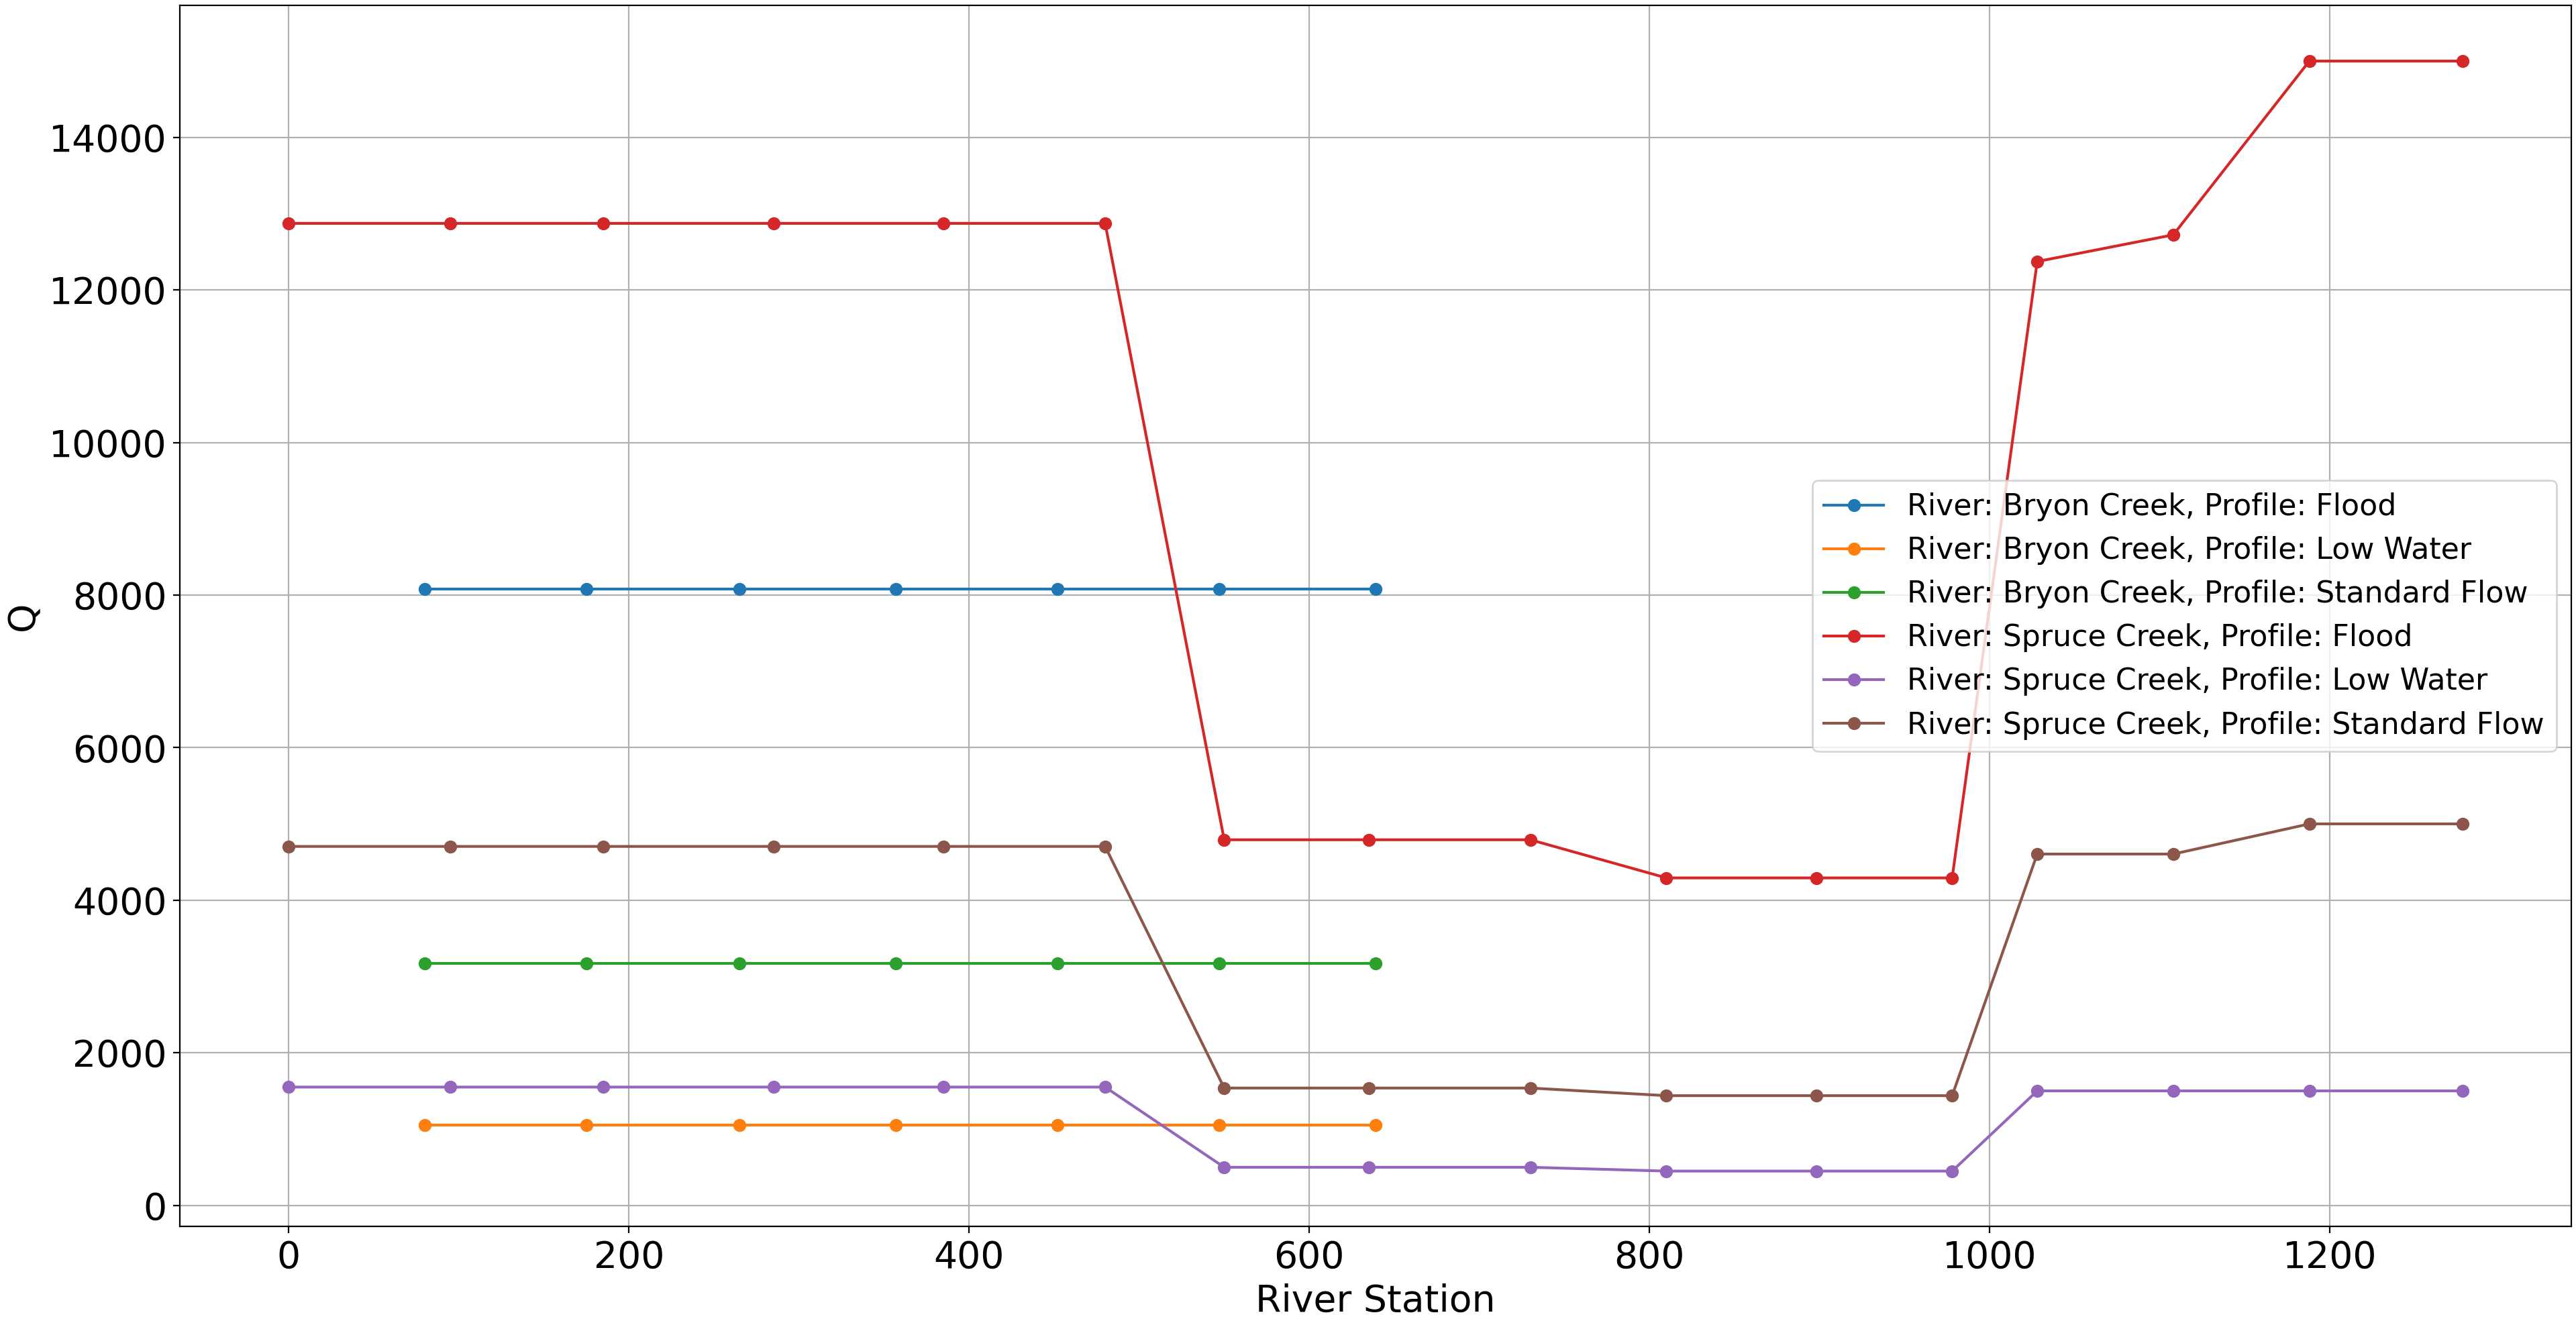
\includegraphics[width=\textwidth]{defaultCase.png}
\end{figure}

\begin{python}
plotHECRAS(riverData, 'Fr')
\end{python}

\begin{figure}[h]
    \centering
    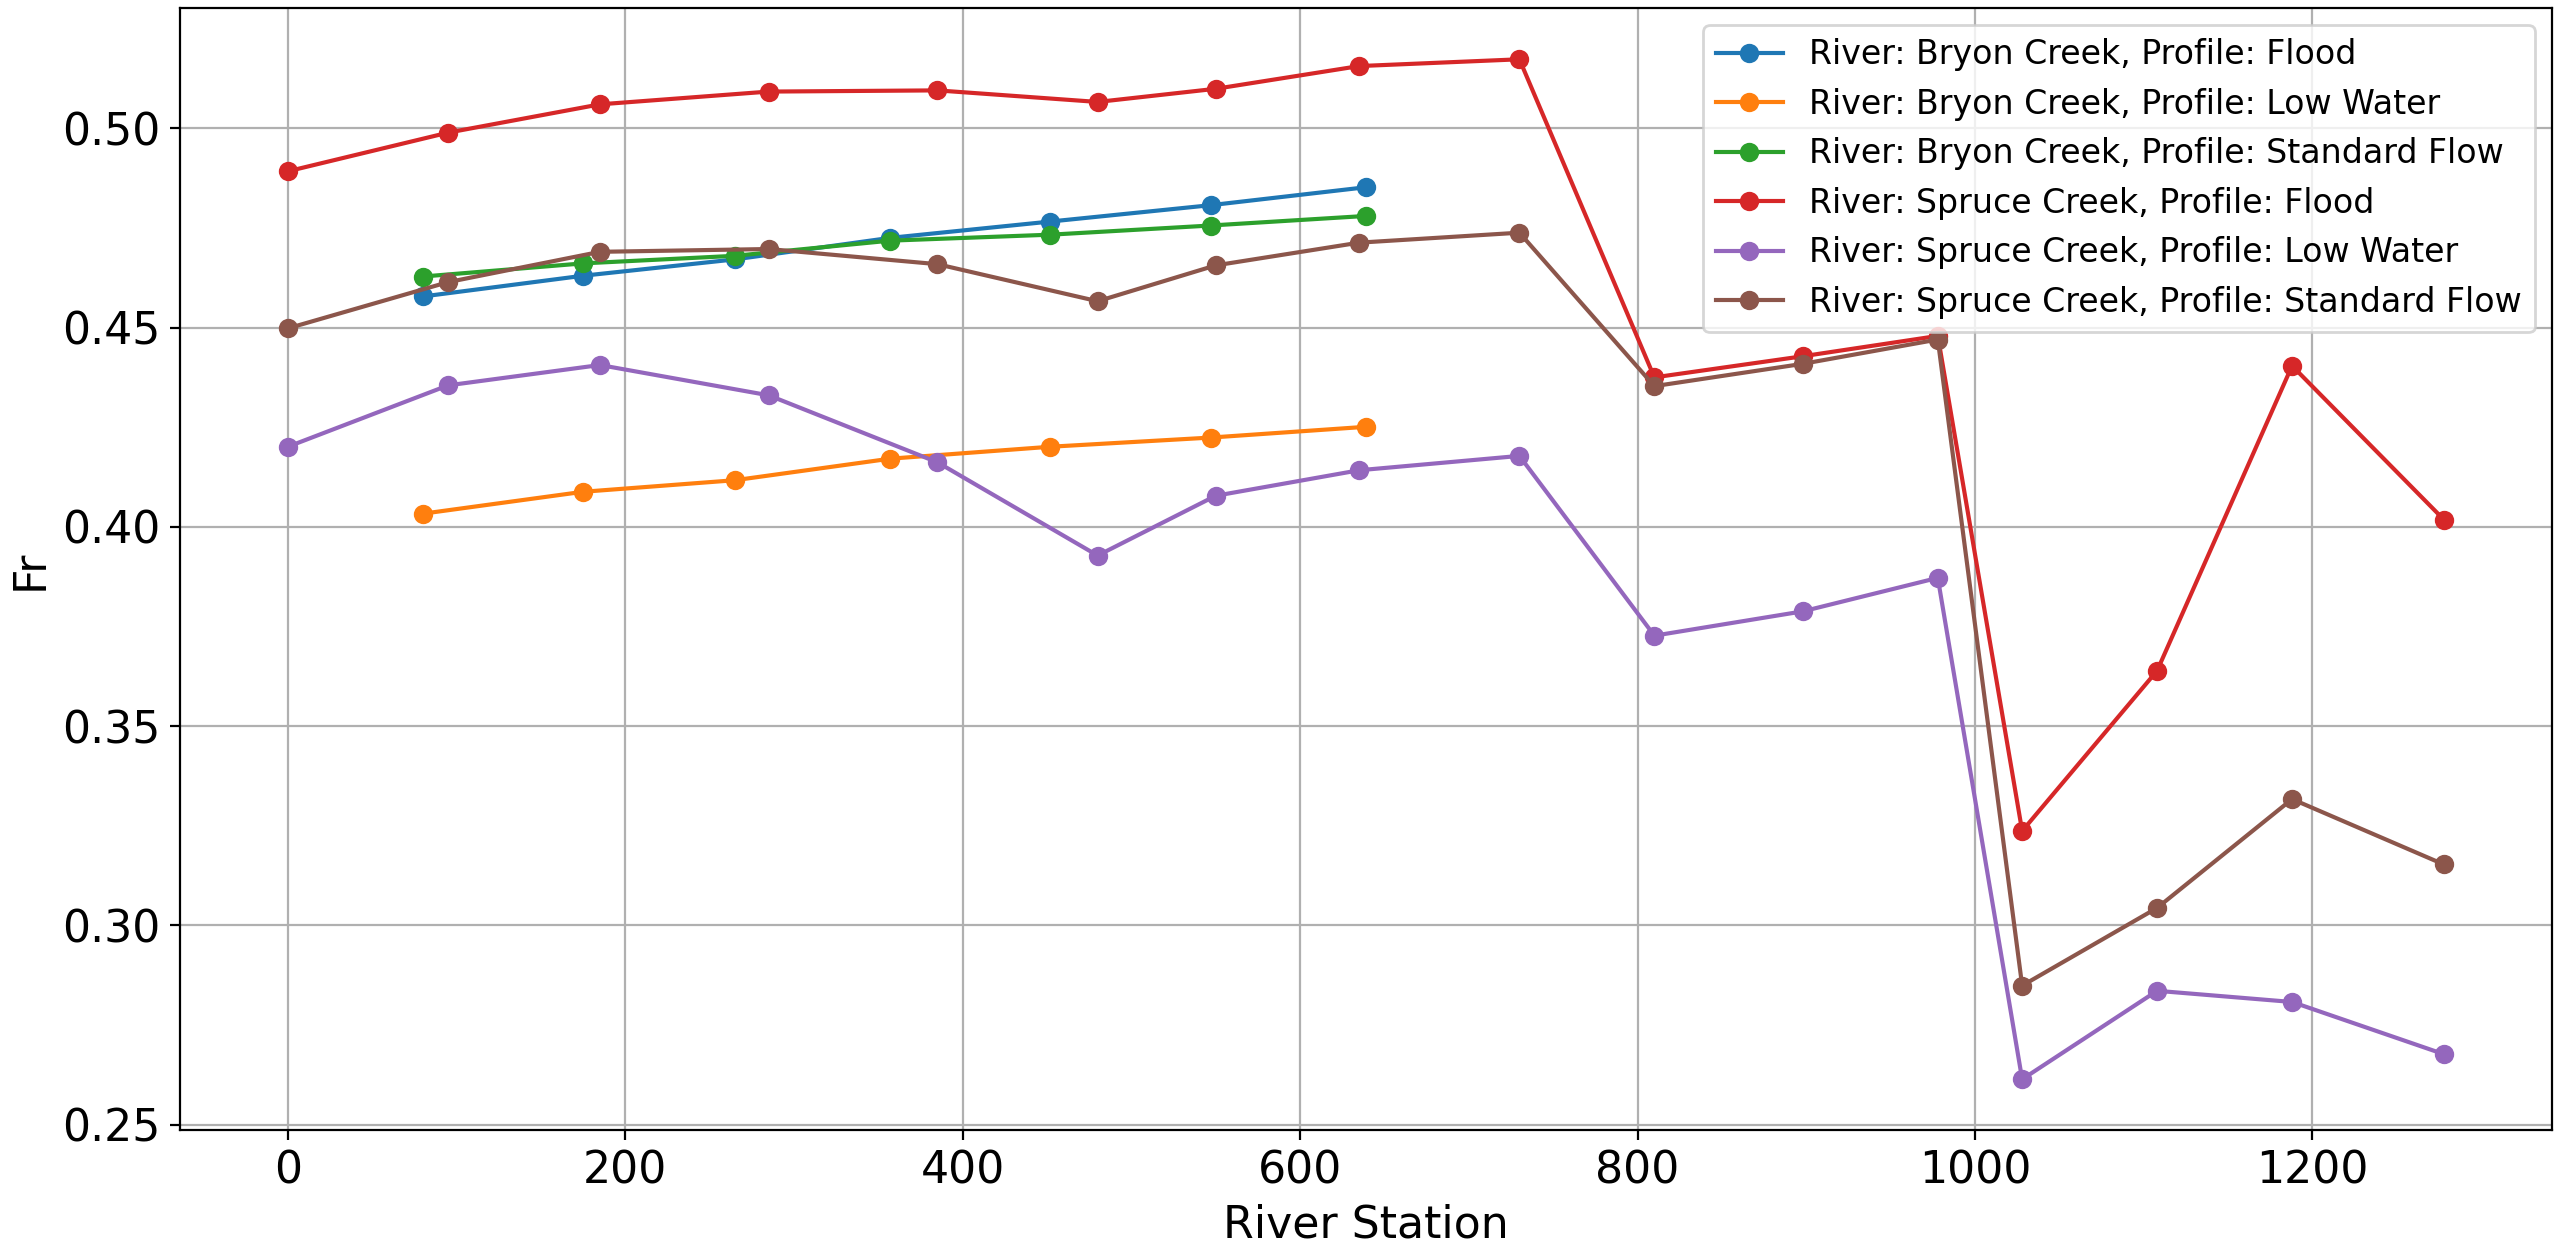
\includegraphics[width=\textwidth]{Fr_allRivers.png}
\end{figure}

\newpage

\section*{Plotting with optional inputs}

\begin{python}
# Plot h for only Bryon Creek
plotHECRAS(df, 'h', riverName='Bryon Creek')
\end{python}

\begin{figure}[h]
    \centering
    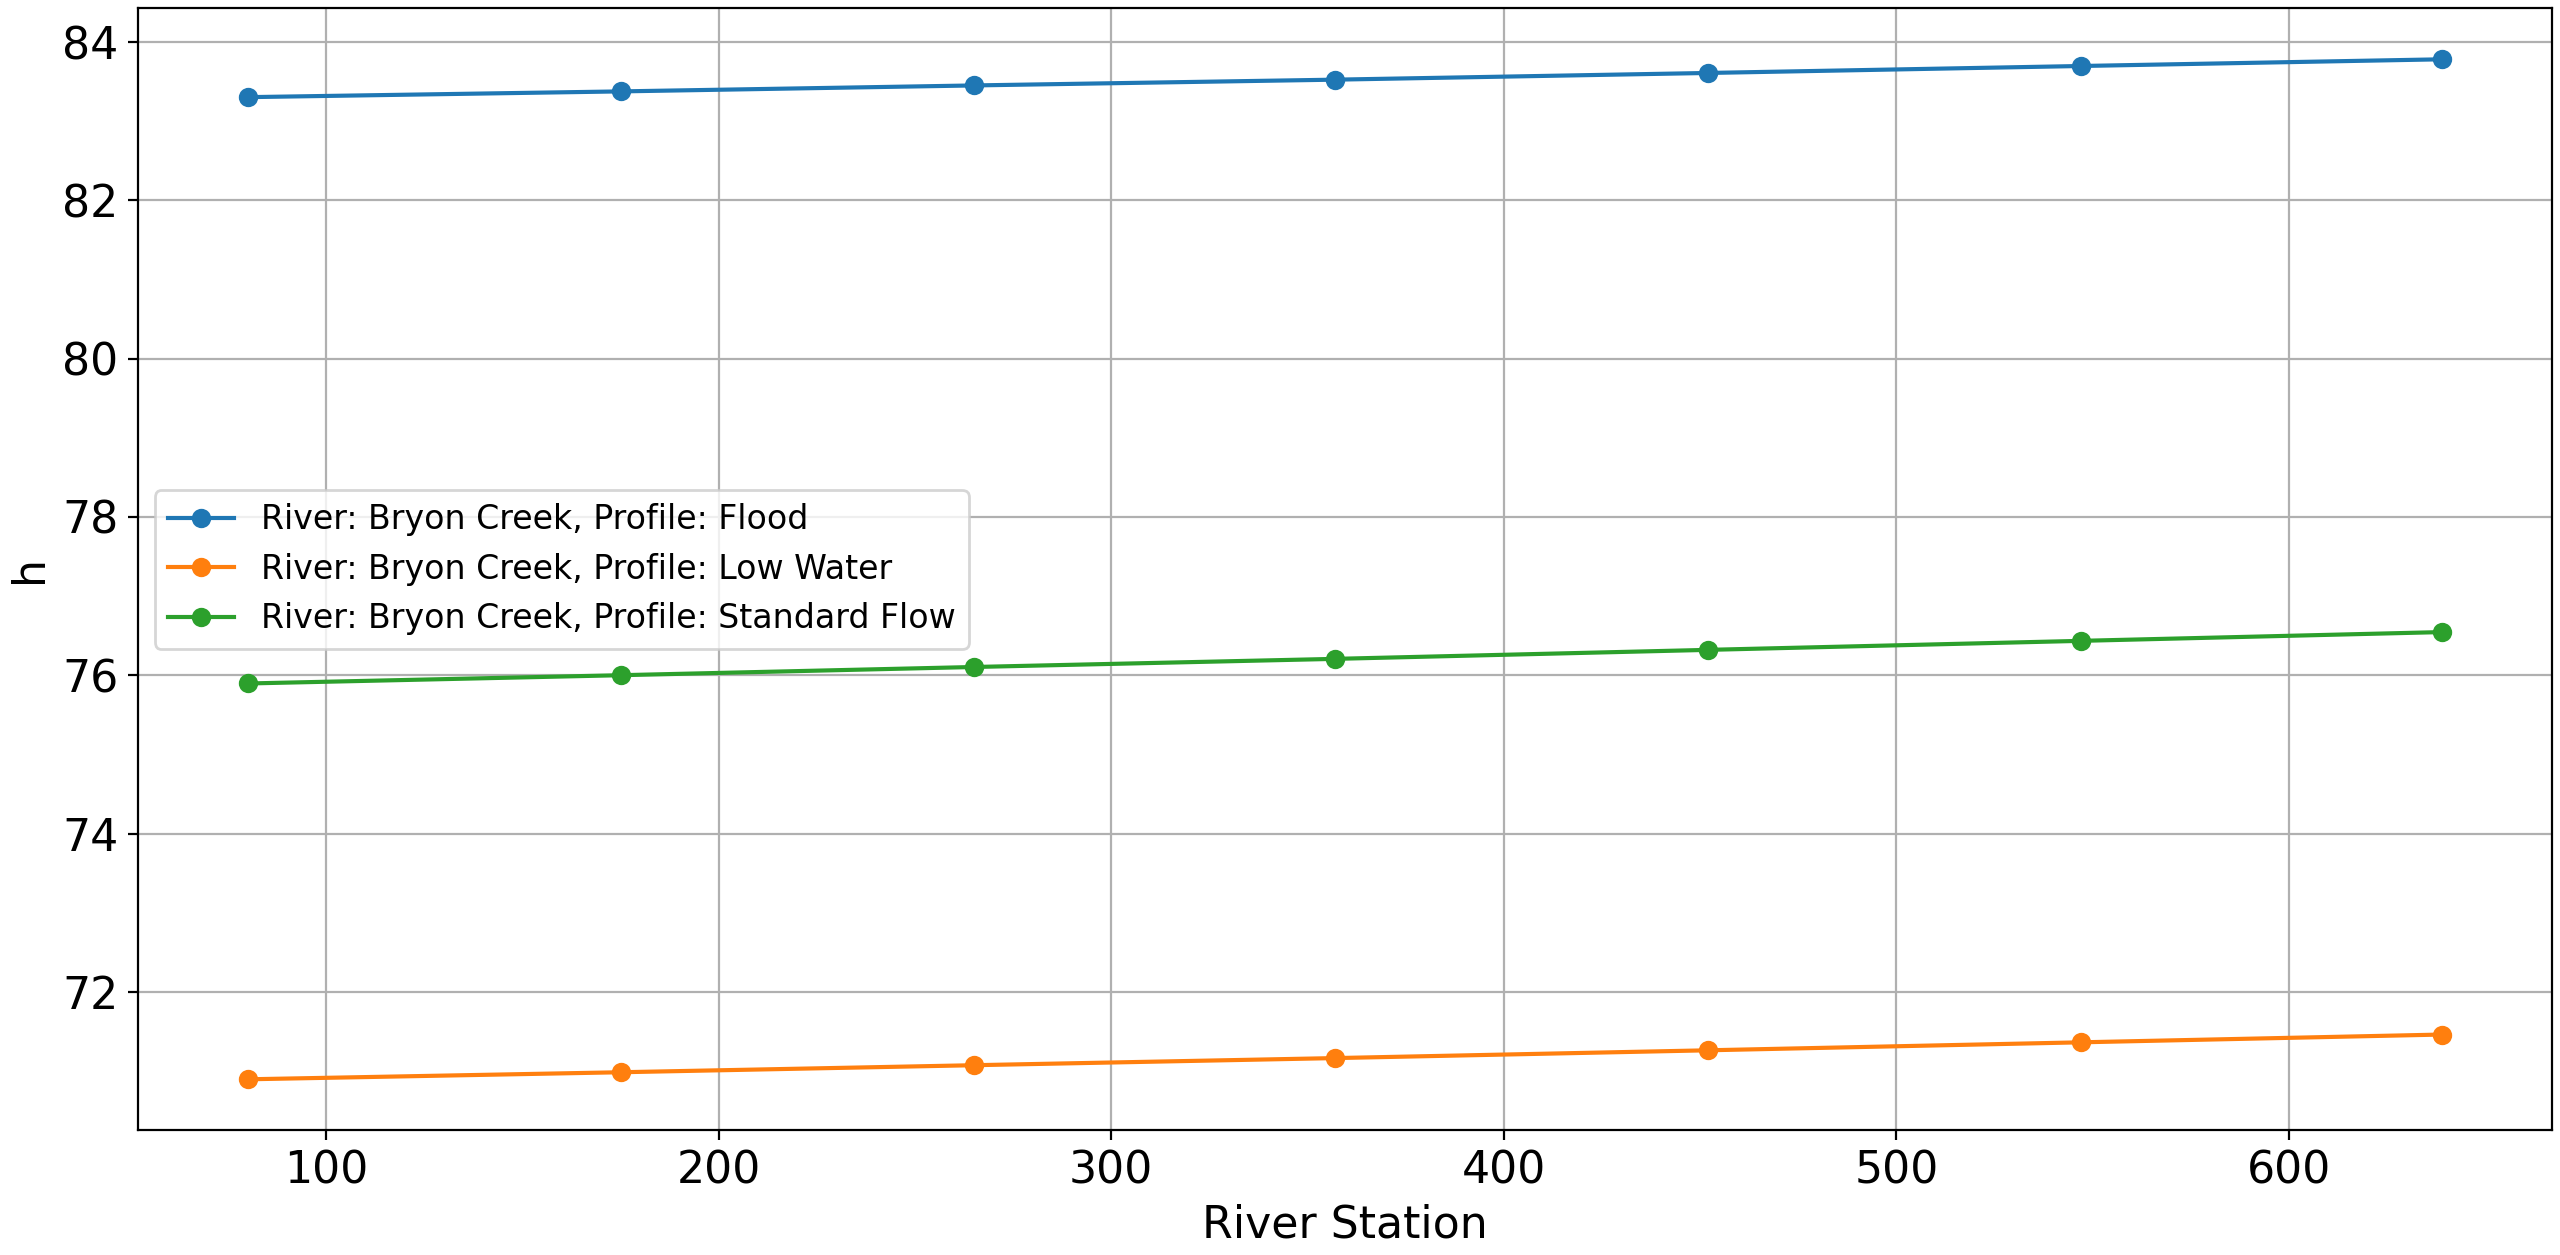
\includegraphics[width=\textwidth]{bryonCreek_h.png}
\end{figure}

\begin{python}
# Plot V for only Spruce creek
plotHECRAS(df, 'V', riverName='Spruce Creek')
\end{python}

\begin{figure}[h]
    \centering
    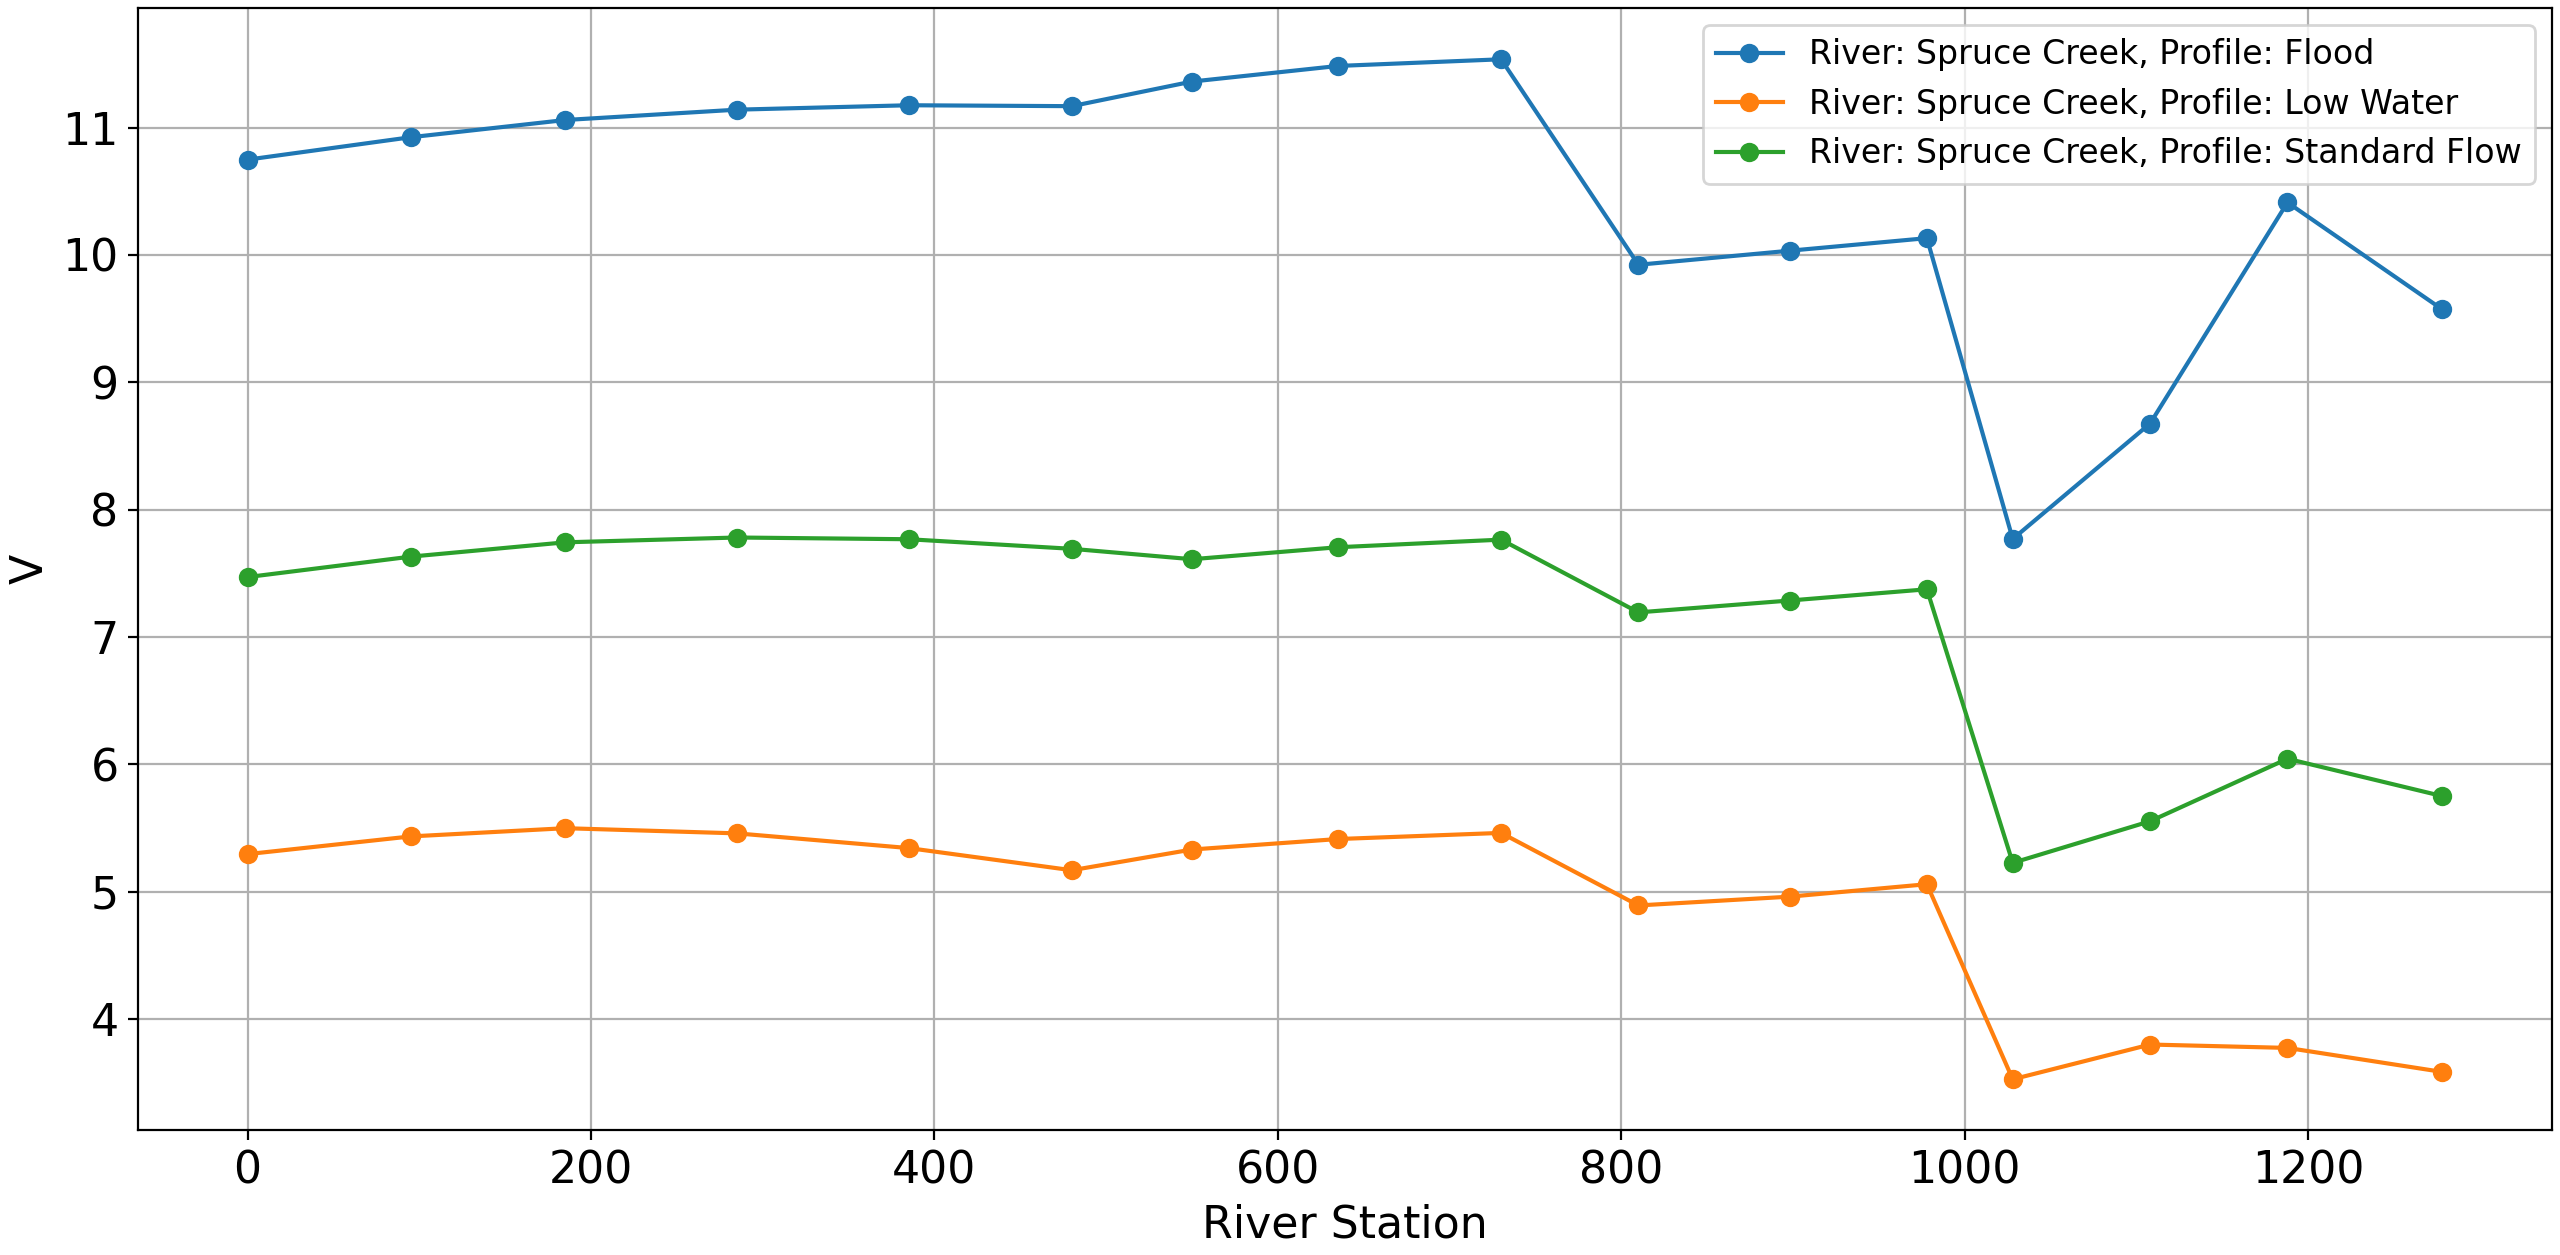
\includegraphics[width=\textwidth]{spruceCreek_V.png}
\end{figure}

\newpage

\begin{python}
# Plot h for Spruce Creek, upper river section
plotHECRAS(df, 'h', riverName='Spruce Creek', 
                    reachName='Upper River')
\end{python}

or, equivalently:

\begin{python}
# Plot h for Spruce Creek, upper river section
plotHECRAS(df, 'h', reachName='Upper River')
\end{python}

\begin{figure}[h]
    \centering
    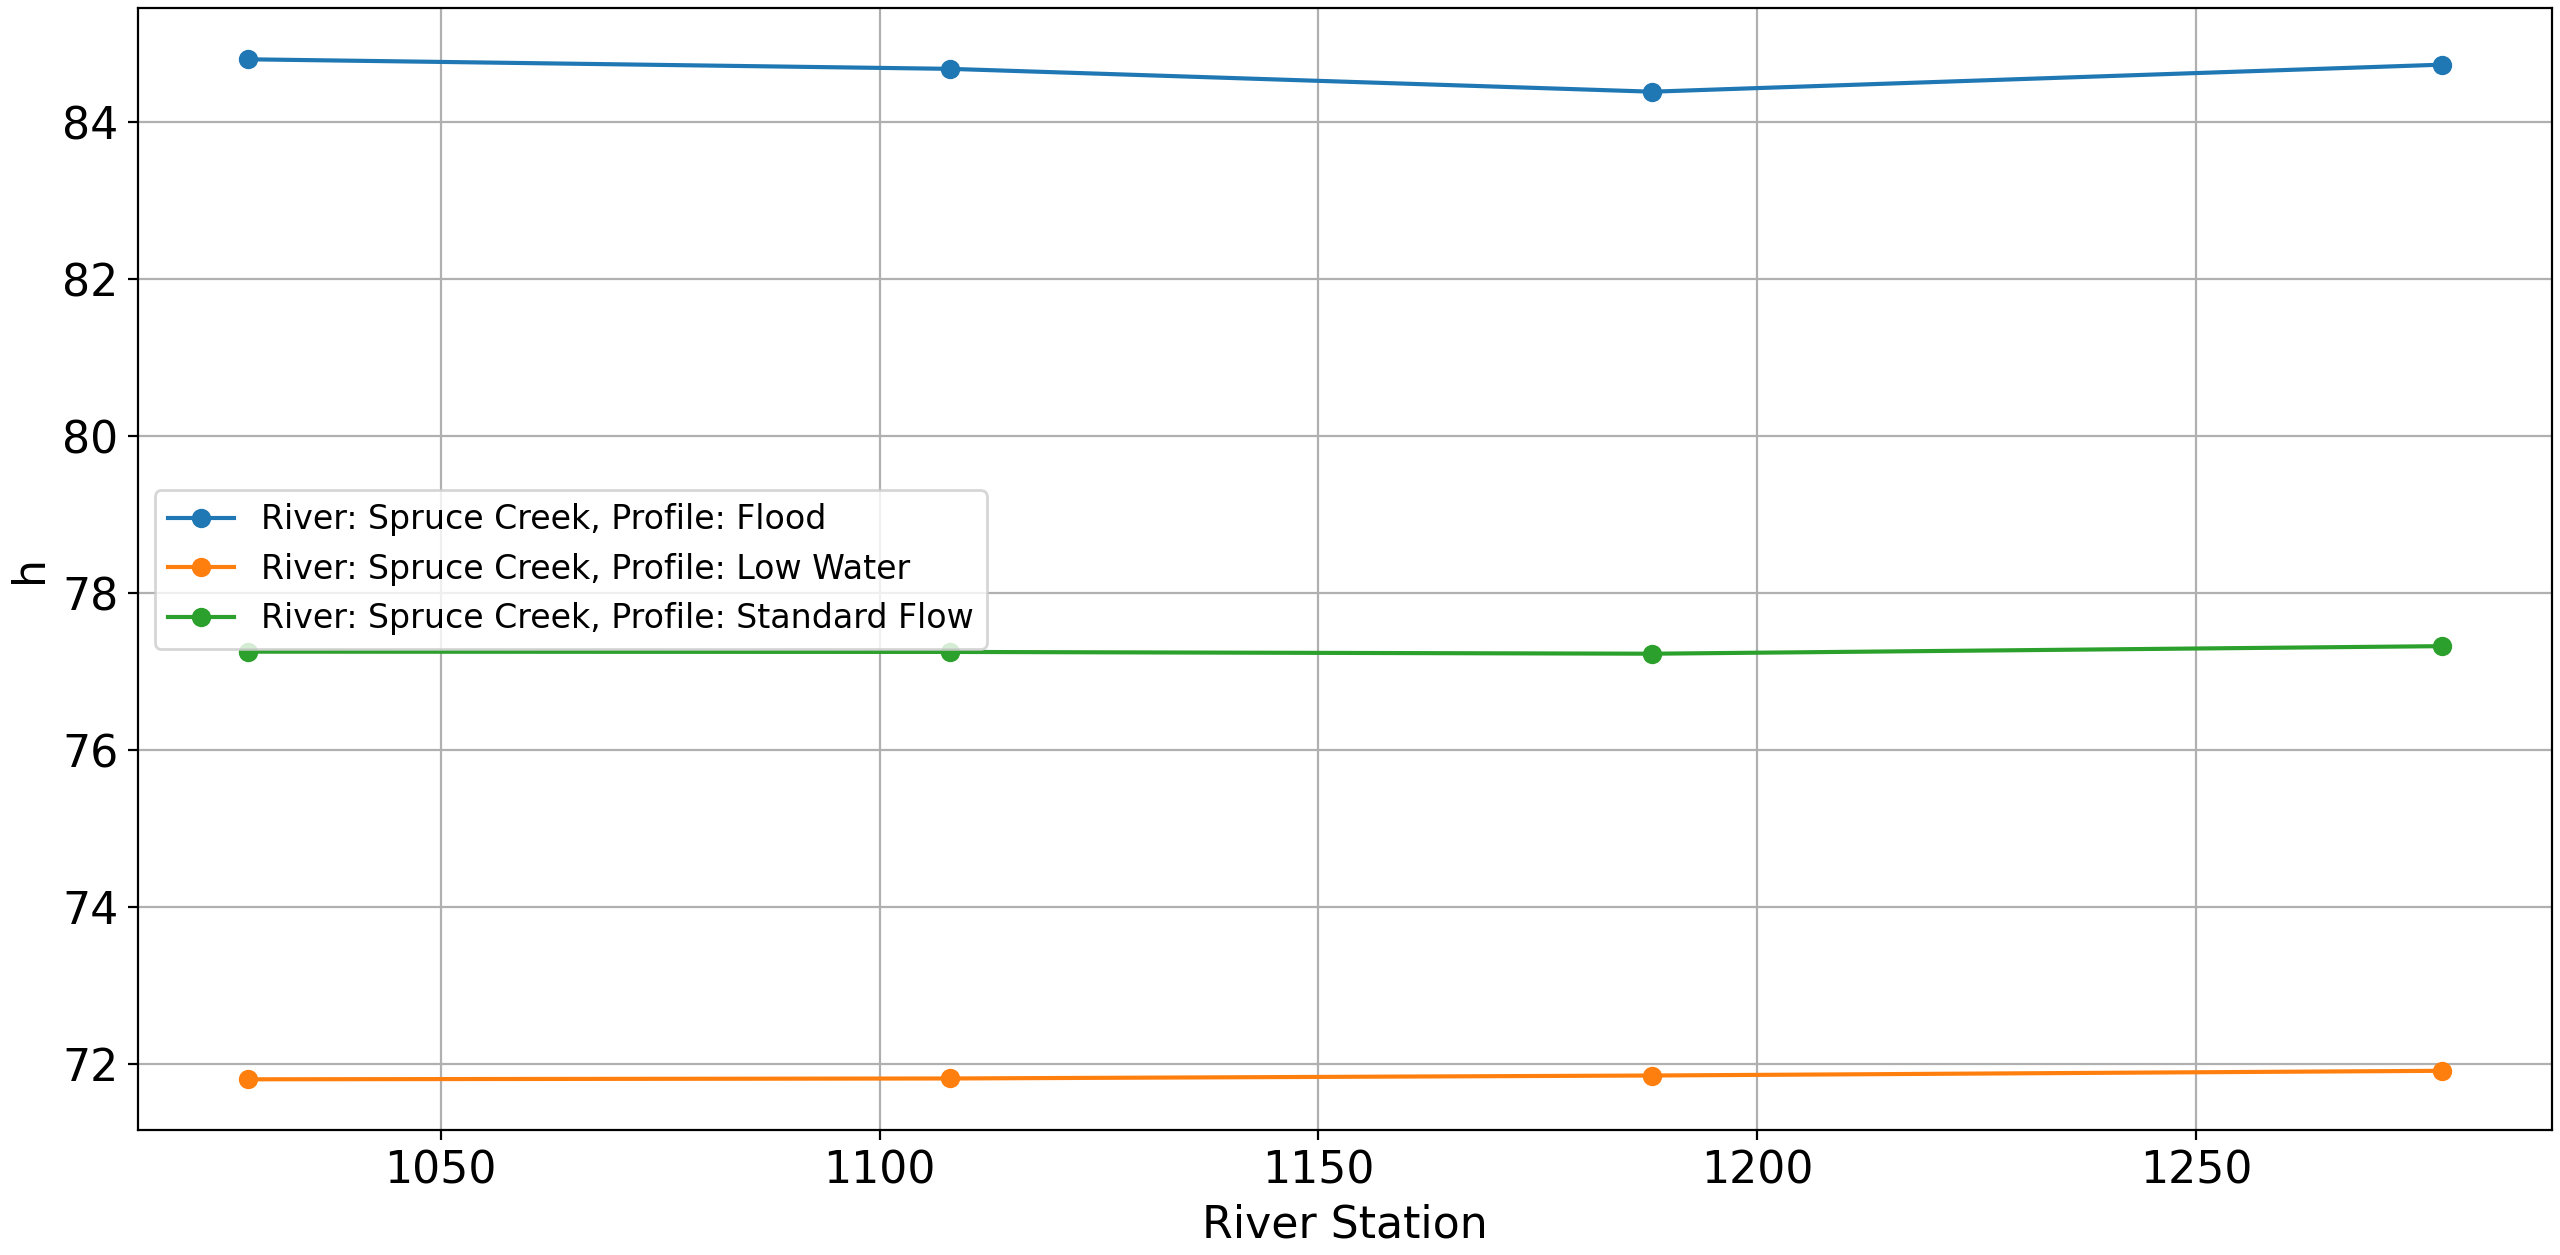
\includegraphics[width=\textwidth]{upperRiver_h.png}
\end{figure}

\begin{python}
# Plot h for Spruce Creek, lower river, flood profile
plotHECRAS(df, 'h', riverName='Spruce Creek', 
                    reachName='Lower River', 
                    profileName='Flood')
\end{python}

\begin{figure}[h]
    \centering
    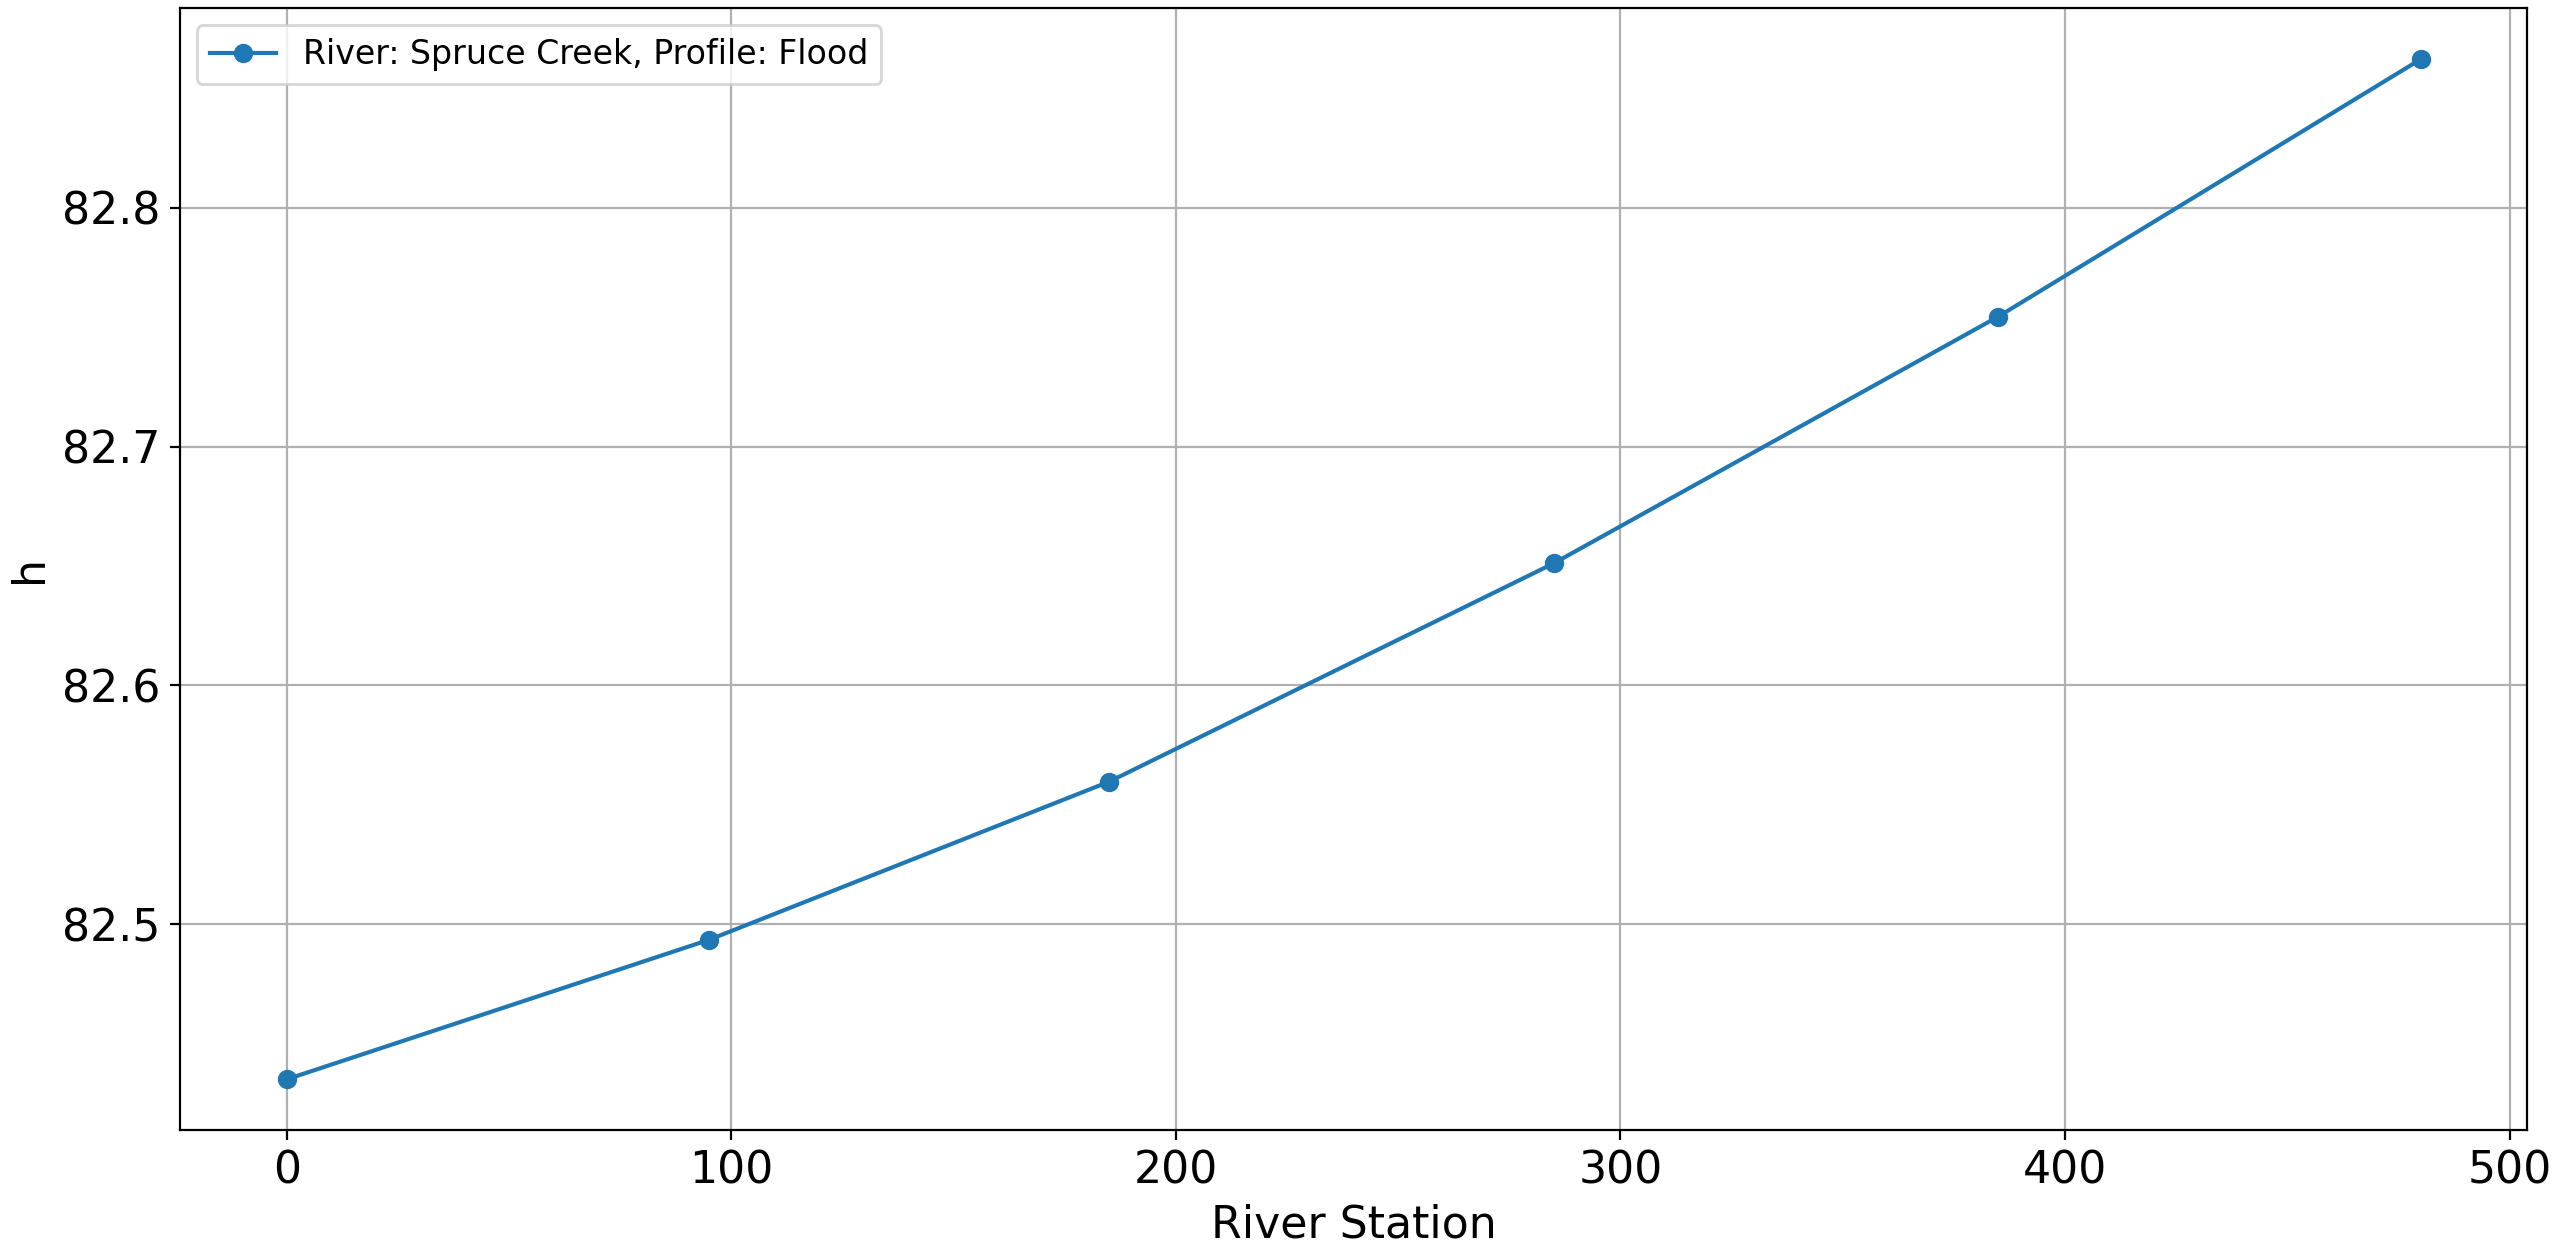
\includegraphics[width=\textwidth]{lowRiverFlood.png}
\end{figure}

\newpage

\begin{python}
# Plot Q for all rivers and reaches, but only low water
plotHECRAS(df, 'Q', profileName='Low Water')
\end{python}

\begin{figure}[h]
    \centering
    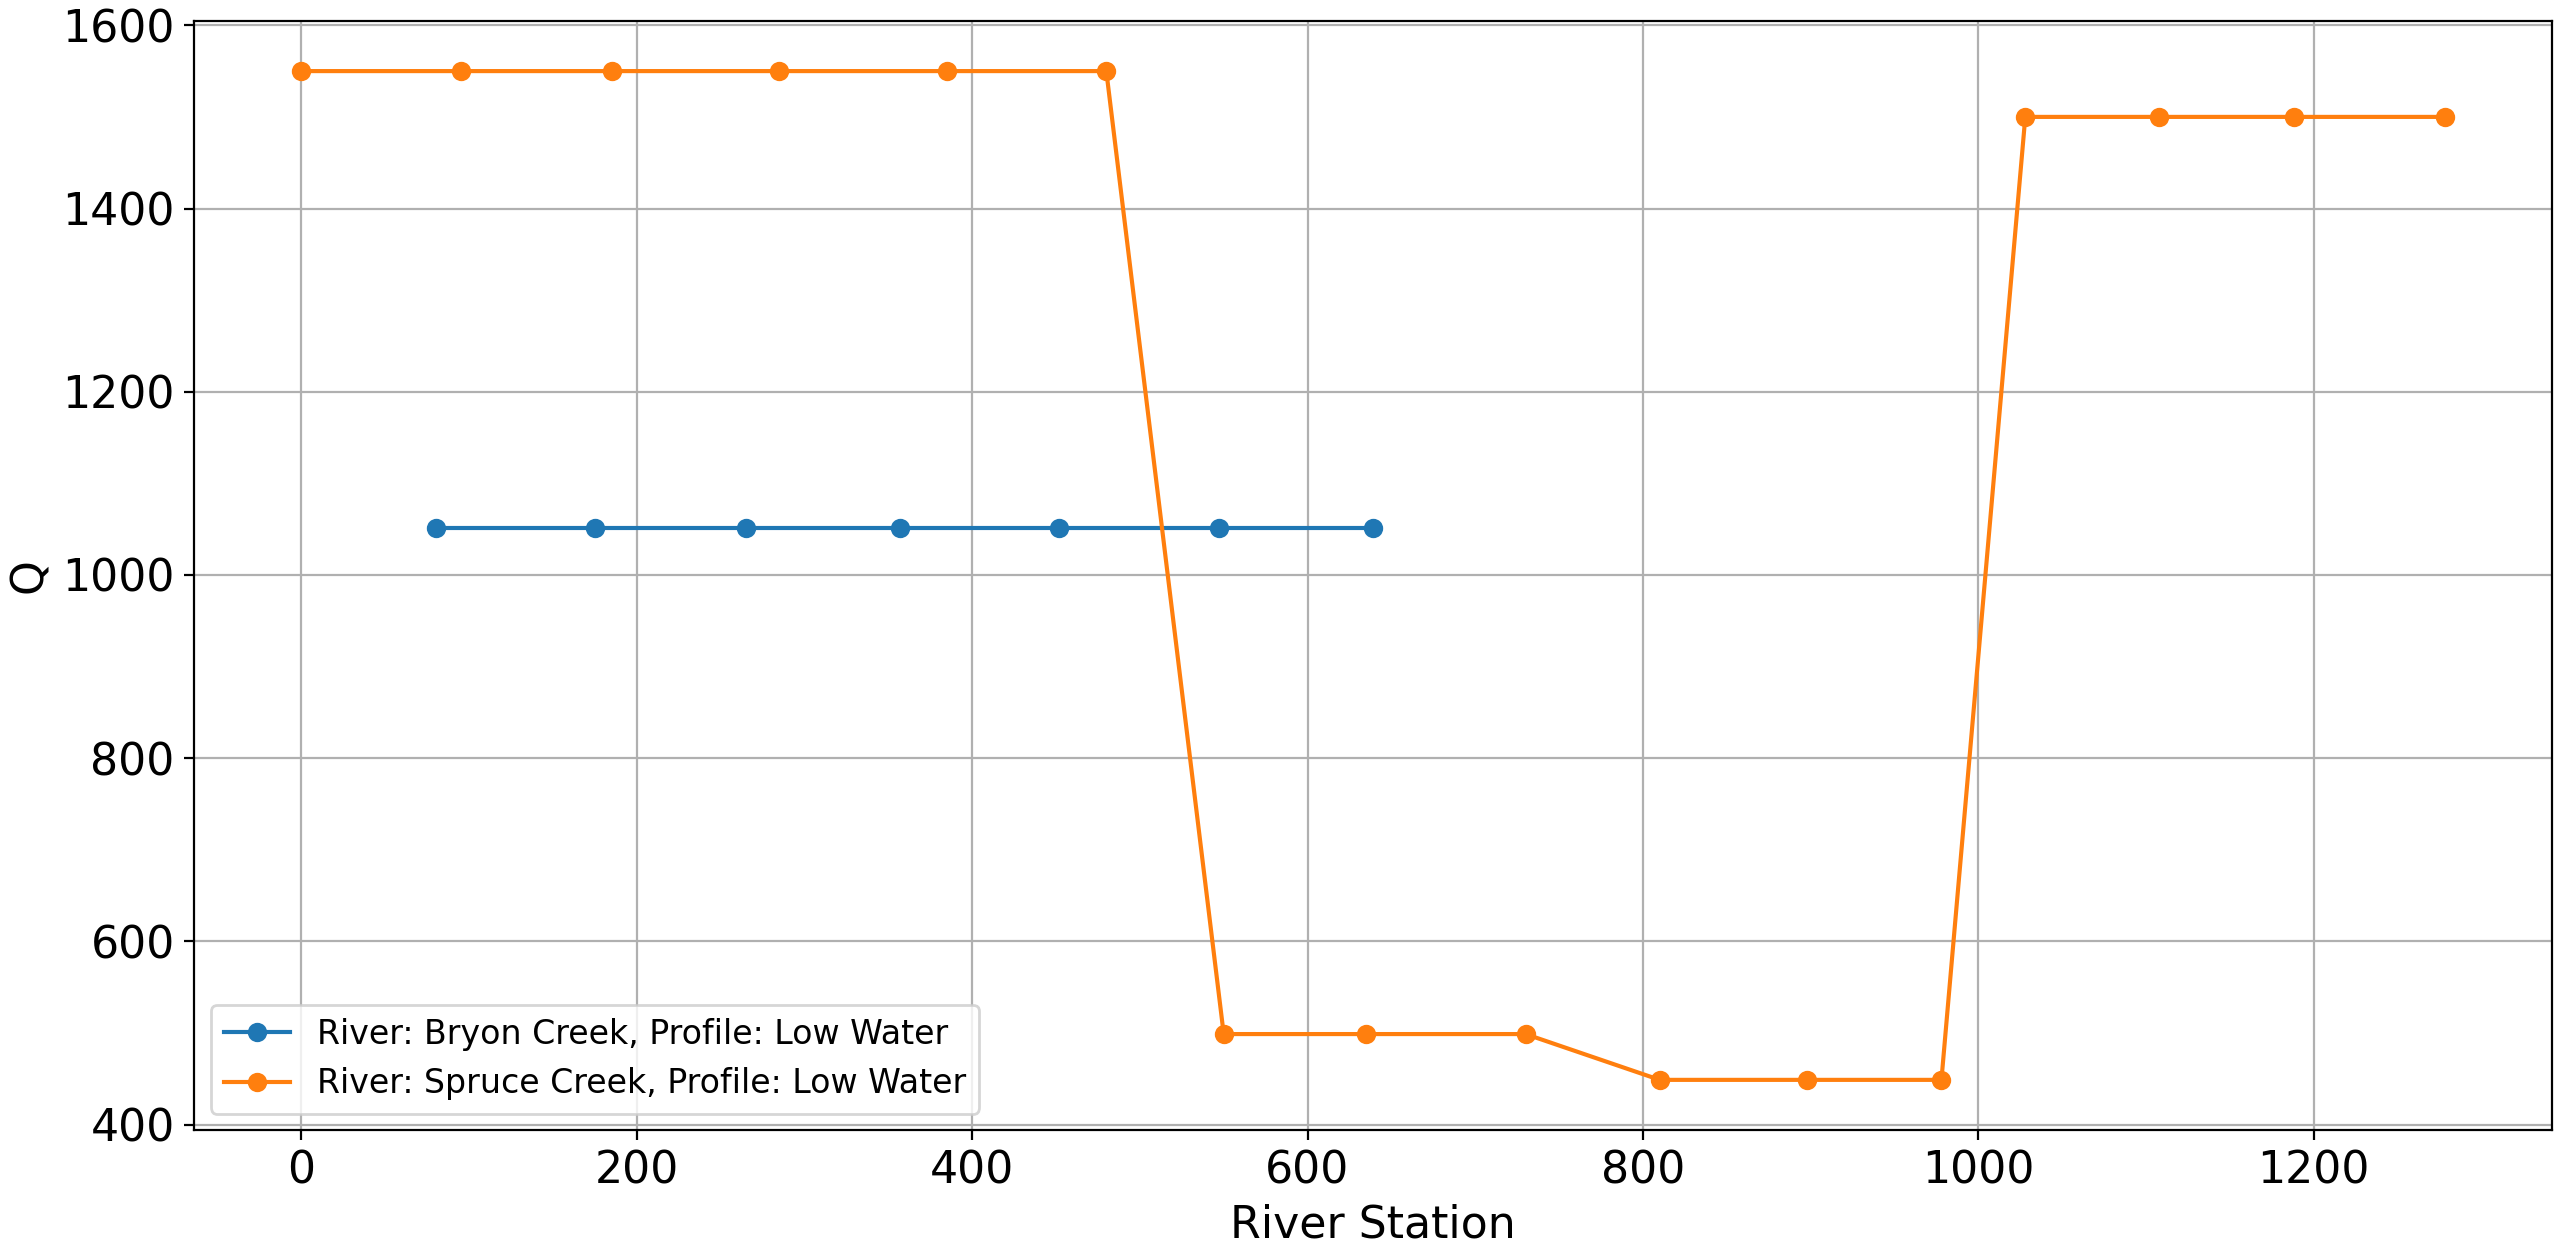
\includegraphics[width=\textwidth]{q_lowWater.png}
\end{figure}

\section*{Example of invalid metric name}
\lstinputlisting[style=BashOutputStyle]{badCol.txt}

\section*{Examples of invalid optional parameters}
\lstinputlisting[style=BashOutputStyle]{badSlice.txt}
\lstinputlisting[style=BashOutputStyle]{badSlice2.txt}

\end{document}